\documentclass[letterpaper,12pt]{article}
\usepackage{tabularx} % extra features for tabular environment
\usepackage{amsmath}  % improve math presentation
\usepackage{graphicx} % takes care of graphic including machinery
\usepackage[margin=1in,letterpaper]{geometry} % decreases margins
\usepackage{cite} % takes care of citations
\usepackage[final]{hyperref} % adds hyper links inside the generated pdf file
\usepackage{float}
\hypersetup{
	colorlinks=true,       % false: boxed links; true: colored links
	linkcolor=blue,        % color of internal links
	citecolor=blue,        % color of links to bibliography
	filecolor=magenta,     % color of file links
	urlcolor=blue         
}
\usepackage{blindtext}
%++++++++++++++++++++++++++++++++++++++++


\begin{document}

\title{DAT510-1 20H Network security and vulnerability. Assignment 1. Cryptanalysis of primitive ciphers}
\author{Asahi Cantu Moreno (student id: 253964)}
\date{\today}
\maketitle

\begin{abstract}
The study of encryption algorithms, techniques and potential vulnerability detection are very important for the understanding and detection of potential risks related to the information transmission over insecure channels. In this assignment a study of the cryptanalysis, the statistical techniques to detect encryption algorithm vulnerabilities and the potential threats of wrong or obsolete algorithms is performed in a two-part code development which involves:
\begin{enumerate}
    \item \textbf{Part I. Polyalphabetic ciphers.} Divided in two different tasks where two ciphered text paragraphs are given to be deciphered by statistical techniques and brute force attacks. Text was ciphered with a poly-alphabetic substitution cipher. Techniques such as word frequency analysis and n-gram frequency analysis are performed to start retrieving the core of the text and eventually find the potential encryption key by knowing the initial parameters of the encryption algorithm. For the second task another ciphered text is analyzed and several keys found by brute-forcing and different decipher techniques which basically consist using the same tools from the first task and special text comparison to find the optimal encryption algorithm.
    \item \textbf{Part II. Simplified DES.} The development of an SDES and triple SDES algorithm provides the insights and abilities to understand how encryption algorithms work under real implementations. Once developed it some keys, plain text and ciphered texts are required to be found, where also special statistical analysis is performed to decipher ciphered messages in order to demonstrate the vulnerability of such encryption mechanism and how these techniques can be easily bypassed by malicious third-parties. Finally the development of a mini web server is performed to analyse the potential vulnerabilities for the encryption algorithm on the back end.
\end{enumerate}
For each element a deep explanation and case study is provided and finally the statistical results of the developed code is presented to provide perspective on the encryption mechanisms studied for this assignment.
The developed code and implementations for each part of the assignment can be found together in the contents of this document repository.
\end{abstract}
\newpage


\section{Part I. Polyalphabetic ciphers.}
Polyaphabetic ciphers are and extension of simple monoalphabetic ciphers where monoalphabetic substitution can be performed by any given letter of the English alphabet (26 letters). The following ciphered text was provided and ciphered with an implementation of the Vigenere Cipher\footnote{The best known, and one of the simplest, polyalphabetic ciphers. The set of related monoalphabetic substitution rules consists of the 26 Caesar ciphers with shifts of 0 through 25. Each cipher is denoted by a key letter, which is the cipher text letter that substitutes for the plain text letter a.\cite{WS2017-Vignere} }: 
\begin{quote}
    BQZRMQ KLBOXE WCCEFL DKRYYL BVEHIZ NYJQEE BDYFJO PTLOEM EHOMIC UYHHTS GKNJFG
EHIMK NIHCTI HVRIHA RSMGQT RQCSXX CSWTNK PTMNSW AMXVCY WEOGSR FFUEEB DKQLQZ
WRKUCO FTPLOT GOJZRI XEPZSE ISXTCT WZRMXI RIHALE SPRFAE FVYORI HNITRG PUHITM
CFCDLA HIBKLH RCDIMT WQWTOR DJCNDY YWMJCN HDUWOF DPUPNG BANULZ NGYPQU
LEUXOV FFDCEE YHQUXO YOXQUO DDCVIR RPJCAT RAQVFS AWMJCN HTSOXQ UODDAG
BANURR REZJGD VJSXOO MSDNIT RGPUHN HRSSSF VFSINH MSGPCM ZJCSLY GEWGQT DREASV
FPXEAR IMLPZW EHQGMG WSEIXE GQKPRM XIBFWL IPCHYM OTNXYV FFDCEE YHASBA TEXCJZ
VTSGBA NUDYAP IUGTLD WLKVRI HWACZG PTRYCE VNQCUP AOSPEU KPCSNG RIHLRI KUMGFC
YTDQES DAHCKP BDUJPX KPYMBD IWDQEF WSEVKT CDDWLI NEPZSE OPYIW
\end{quote}

It can be assumed that the cipher technique used only lowercase letters as key transformation and the spaces were removed during the encryption process. It was finally split into 8-char segments and transformed to uppercase for better readability. Therefore three basic factors are to be assumed:

\begin{enumerate}
    \item The text was ciphered using only lower characters from the English Alphabet
    \item The spaces for the encoded text were removed
    \item There is no special char other than English alphabet letter present in the plain text.
    \item A key no longer than 10 characters was used to encrypt the message
\end{enumerate}

\subsection{Ciphered text statistical analysis}
Before any statistical analysis can be performed it is necessary to highlight the importance of statistical English alphabet such as\cite{lettfreq}:

\begin{itemize}
    \item English letter frequency distribution
    \begin{quote}
        e t a o i n s r h l d c u m f p g w y b v k x j q z
    \end{quote}
    \item 2-gram frequency distribution
    \begin{quote}
         th he an in er on re ed nd ha at en es of nt ea ti to io le is ou ar as de rt ve
    \end{quote}
    \item 3-gram frequency distribution
        \begin{quote}
        the and tha ent ion tio for nde has nce tis oft men
        \end{quote}
\end{itemize}

It is very important for a cryptanalysis to start with a strong basis and assumptions about the alphabet that might have been used and the language since it can give big insights for the pattern detection of ciphered words being together representing either a letter, a 2-gram and even a 3-gram.

With this pattern in mind it is feasible to perform a statistical analysis on based on the estimated frequency some words or n-grams can appear in a sentence such an in the following example:

\begin{figure}[H]
    \centering
    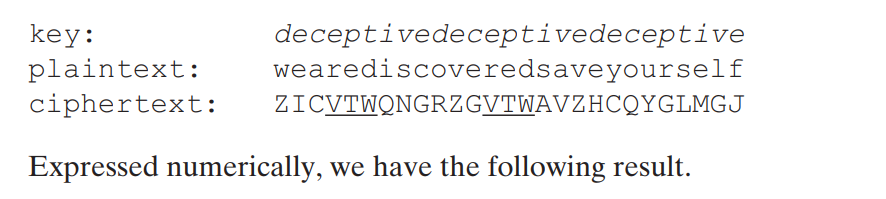
\includegraphics[width=.7\textwidth]{assets/cypher_book.png}
    \caption{Cryptanalysis of a simple sentence showing the pattern repetition of ciphered words for a predefined phrase\cite{WS2017-Vignere}}
\end{figure}

\blindtext %delete this line

Bi performing a statistical analysis with python code on the ciphered text it was possible to find the following patterns:
\begin{figure}[H]
    \centering
    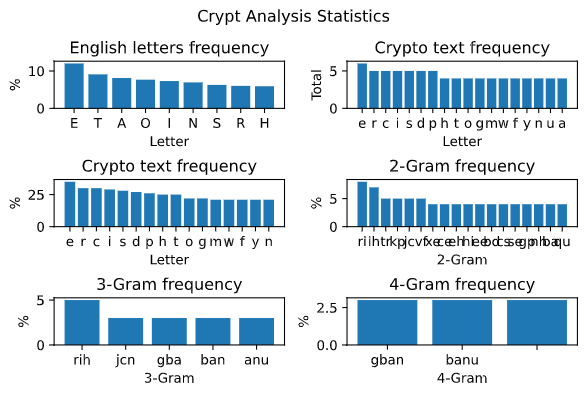
\includegraphics[width=1\textwidth]{assets/cryptstatistics.png}
    \caption{Statistical word, 2-gram and 3-gram distribution on the ciphered text}
\end{figure}

And then with such assumptions it was possible to create a dictionary with the candidate patterns set in the ciphered text:
\begin{figure}[H]
    \centering
    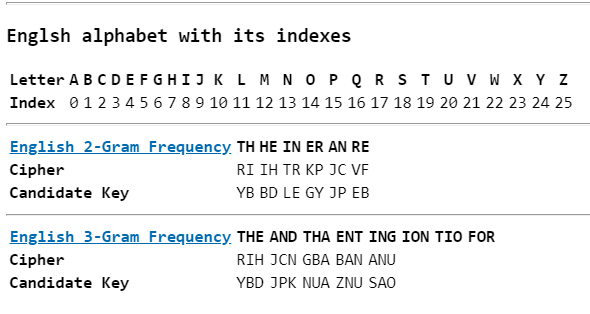
\includegraphics[width=0.8\textwidth]{assets/CryptStatisticsDict.png}
    \caption{Potential 2-gram and 3-gram pattern detected in the ciphered text.}
\end{figure}

Taking into account the 2-gram 'TH'(Which is a candidate for ciphered pattern 'RI') and 3-gram 'THE' (which is also a candidate for ciphered pattern 'RIH') the candidate fragment of the key is found to be \textbf{'YBD'}.

From this approach and trying to find a repetitive pattern with the provided keys, a special fragment of the ciphered text (which contained the pattern 'RI') was chosen to perform a brute-force key analysis. The created algorithm intended to find first the key length by increasing the key size and trying to spot potential English fragments after running up to a 10 length key.

With an 8-length key 'YBDaaaaa' very plausible phrases were found.

\begin{figure}[H]
    \centering
    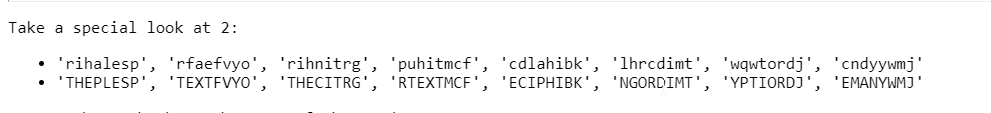
\includegraphics[width=0.8\textwidth]{assets/bruteforce.png}
    \caption{Final insight for a potential candidate pattern with key = 8-char length with repetitive english words.}
\end{figure}

For the rest of the analysis some candidate composed words were guessed to be present in the phrase and then the brute force algorithm was run several times to confirm the hypothesis whether a special key-char could be present and chosen on purpose as well to reduce the brute-force time consumption.

After several trials the key '\textbf{'bdlaekcy'}' was successfully found with th decipher text from the original message:

\begin{quote}
    AN ORIGINAL MESSAGE IS KNOWN AS THE PLAIN TEXT WHILE THE CODED MESSAGE IS CALLED THE CIPHERTEXT. THE PROCESS OF CONVERTING FROM PLAIN TEXT TO CIPHER TEXT IS KNOWN AS ENCIPHERING OR ENCRYPTION RESTORING. THE PLAIN TEXT FROM THE CIPHER TEXT IS DECIPHERING OR DECRYPTION. THE MANY SCHEMES USED FOR ENCRYPTION CONSTITUTE THE AREA OF STUDY KNOWN AS CRYPTOGRAPHY SUCH A SCHEME IS KNOWN AS A CRYPTOGRAPHIC SYSTEM OR A CIPHER TECHNIQUES USED FOR DECIPHERING A MESSAGE WITHOUT ANY KNOWLEDGE OF THE ENCIPHERING DETAILS FALLIN TO THE AREA OF CRYPTANALYSIS. CRYPTANALYS IS IS WHAT THE LAY PERSON CALLS BREAKING THE CODE. THE AREAS OF CRYPTOGRAPHY AND CRYPTANALYSIS TOGETHER ARE CALLED CRYPTOLOGY.
\end{quote}

It is possible to check and confirm this is the key by running a polyalphabetic algorithm with the provided key and trying to match it with he initial ciphered pattern.

Finally it was required for the algorithm to encrypt the same text with an increasing key length and measure the time that the algorithm took to encrypt the phrase with longer keys. The results were very interesting:
\begin{figure}[H]
    \centering
    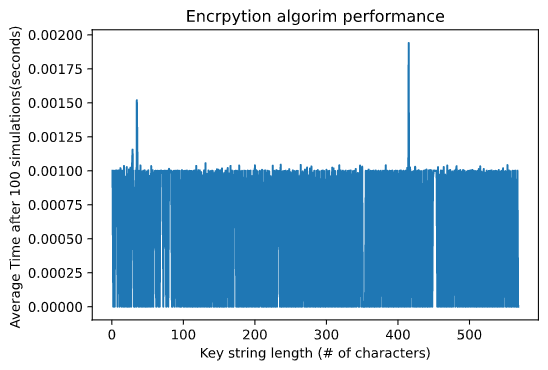
\includegraphics[width=0.7\textwidth]{assets/timeconsumption.png}
    \caption{Performance measure of time taken to encrypt the same text with longer keys.}
\end{figure}

It was initially thought that the time would increase as the key-length was bigger, however, regardless the key size the algorithm took approximately the same amount of time.

\subsection{Complex Ciphered text statistical analysis }
Another ciphered text was provided. Same algorithm and key used to decipher the previous message were employed in the original encryption method.It was necessary to find the additional pattern done to the algorithm that allowed the decryption of the given ciphered sentence:

\begin{quote}
BQZRMQ KLAYAV AYITET EOFGWT EALRRD HNIFML BIHHQY XXEXYV LPHFLW UOJILE GSDLKH
BZGCTA LHKAIZ BIOIGK SZXLZS UTCPZW JHNPUS MSDITN OSKSJI EOKVIL BKMSZB XZOEHA
KTAWXP WLUEJM AIWGLR TZLVHZ SATVQI HZWAXX ZXDCIV TMLBIQ RWZMLB VNGVQK AIZBXZ
HVVMMA MJLRIW GKITZL VHZRRV YCBTVM FVOIYE FSKGKJ AVWHUV BUHZSA EFLHMQ HHVSGZ
XIKYTS YZXUUC KBTOGU VABLDP BGJCGF NLIIYA HJFWGG PSCPVA ZEASME MLGOYR CGFXVG
EJTTTW TSAAIL QFKEEP CPULXW WZRLVI VVYUMS MSILRI IBLWJI TKWUXZ GUZEJG DUCQEE
QEOBTP SIHTGW UALVMA ILTAEZ TFLDPE IVEGYH PLZRTC YJVYGX ABFNPQ XLCEYA RGIFCC WHBGIF
WSYLBZ MDWFPX KZSYCY APJTFR CKTYYU YICYLR ZALETS DWHMGR PTTGUW CGFNTB JTRNWR
AADNPQ XLTBGP RZMJTF KGTSPV DTVAPE ZPRIP
\end{quote}

It was very interesing to notice (not after decrypting unfortunately) that the first 8 characters of the decrypted text matched the first character from the previous deciphered message.

\begin{quote}
    \textbf{anorigin}zvpvwogvdqtobwuvdxarntfphcblxyfj...
\end{quote}

It was then a matter to figure out how the key was used to encrypt the rest of the message. Finally and after several trials it was found that for this message the first 8 characters were encoded with the initial key, but the second segment could be decoded by using the previous encoded pattern as a key.

The final deciphered text turned out to be the same as the first one.

\section{Part II. Simplified DES.}
In this section it was required to implement an SDES and triple-DES algorithm to find the keys and ciphered text combinations.

\subsection{SDES Tests}
\begin{figure}[H]
    \centering
    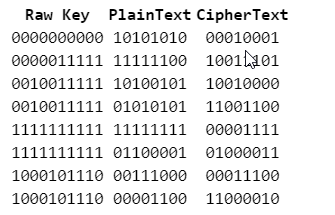
\includegraphics[width=0.5\textwidth]{assets/SDES_Test.png}
    \caption{Test performed with the implemented SDES algorithm.}
\end{figure}

\subsection{Triple SDES Tests}
\begin{figure}[H]
    \centering
    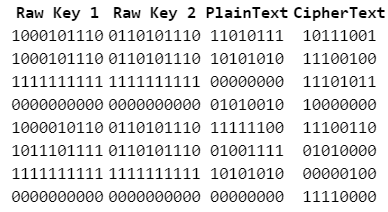
\includegraphics[width=0.5\textwidth]{assets/3SDES_Test.png}
    \caption{Test performed with the implemented Triple SDES algorithm.}
\end{figure}

\subsection{SDES Text Cracking}
\begin{figure}[H]
    \centering
    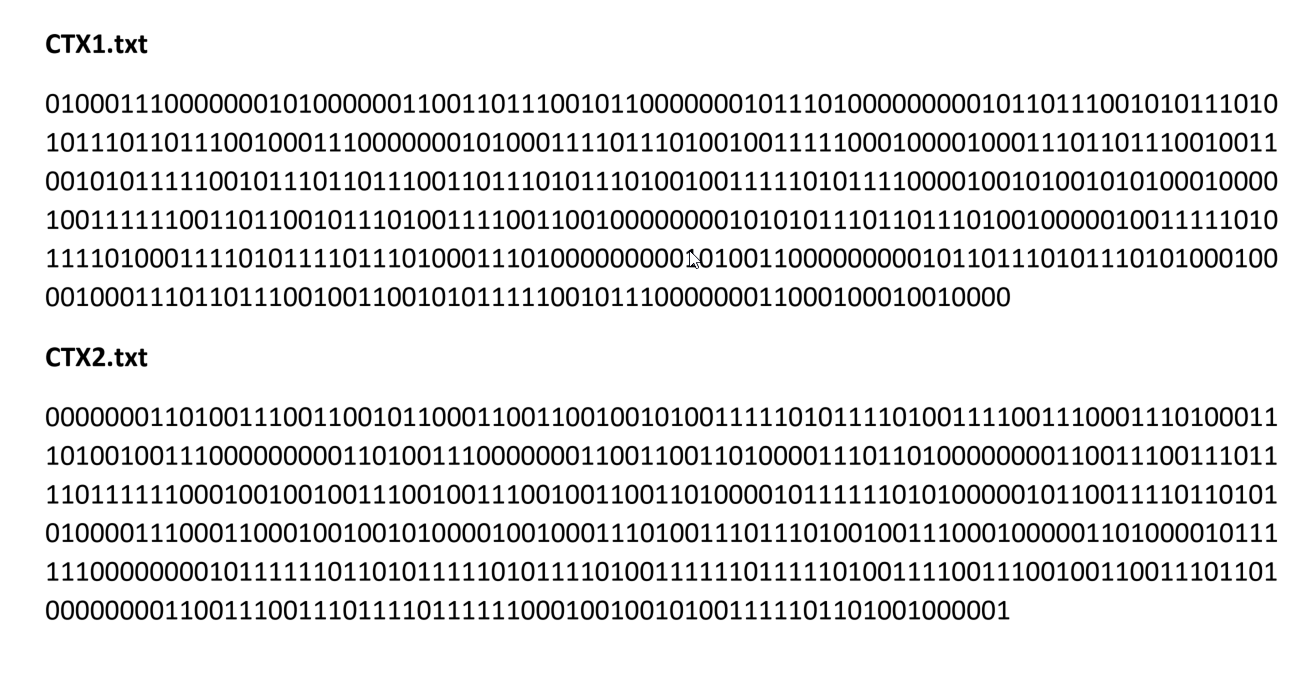
\includegraphics[width=0.7\textwidth]{assets/CipherText.png}
    \caption{Provide texts to be deciphered with SDES and triple SDED respectively.}
\end{figure}
A ciphered text was provided and key required to be found given the same conditions as in part 1. To find he candidate key the same statistical method was applied with he intention to find all the potential ciphered segments that would math the character 'e' (since 'e' is the most common letter in the alphabet. The most frequent token 8-bit segments were chosen to be deciphered with an increasing key and then try to find if by deciphering such segment the result was and 'e' or 'E'. If that happens then decipher the rest of the message and check for non-alphabet characters, which in such case would be assumed to be an invalid deciphered text and discarded.

The increasing key would go from '0000000000' to '1111111111' (1024 permutations or $2^{10}$). Also, first 5 most frequent 8-bit patterns were chosen to be run against the brute-fore attack, the maximum amount of instructions to run would be $1024*5=5120$ cycles to find the potential deciphered text, something meaningless in terms of resource consumption. The found key is  \textbf{1111101110} and deciphered message \begin{quote}simplifieddesisnotsecureenoughtoprovideyousufficientsecurity\end{quote}. 

\begin{figure}[H]
    \centering
    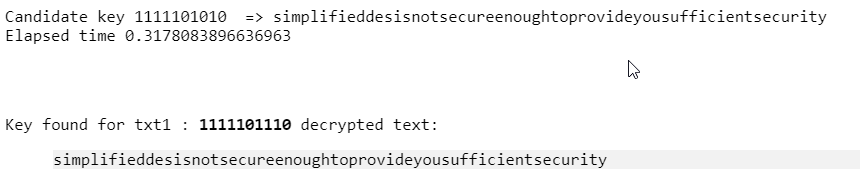
\includegraphics[width=0.7\textwidth]{assets/SDESCrack.png}
    \caption{Deciphered text and time consumption for SDES message deciphering.}
\end{figure}

\subsection{Triple SDES Text Cracking}
A new ciphered text message was provided and asked to find the ciphering keys. Same procedure is performed as in previous task with the difference that triple SDES uses two 10-bit key segments, so now the maximum amount of instructions to run would be $1024*1024*5=26214400$ cycles to find the potential deciphered text. This is 5120 more trials required to find candidate keys. The found key is  \textbf{k1=1111101010, k2=0101011111} and deciphered message \begin{quote}simplifieddesisnotsecureenoughtoprovideyousufficientsecurity\end{quote}. 

\begin{figure}[H]
    \centering
    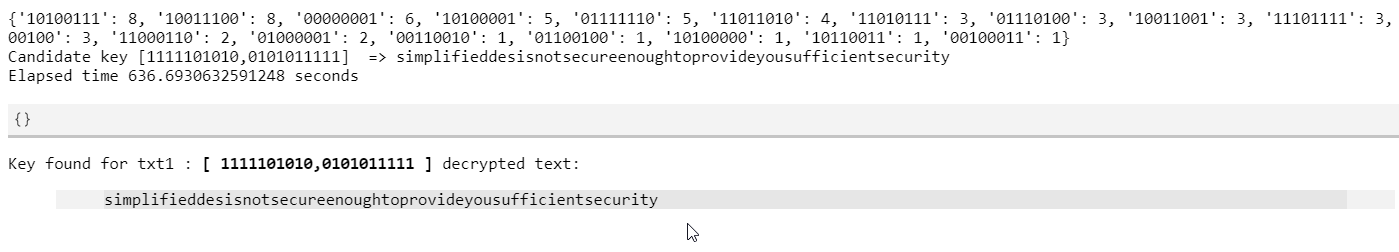
\includegraphics[width=0.7\textwidth]{assets/3SDESCrack.png}
    \caption{Deciphered text and time consumption for Triple SDES message deciphering.}
\end{figure}


\subsection{Server implementation for messaging ciphering/deciphering}
A mini web server was implemented with Flask-Python. Built SDES and Triple SDES algorithms were implemented to decrypt and encrypt a given message via a web page. The keys were provided (k1 ='1000101110', k2='0110101110') and store in raw text on the back-end side of the server, which means that a malicious user would not be able to spot the key unless he has access to the source code  of the solution. It has also been highlighted from previous deciphering mechanisms that not much computational resources would be required to eventually crack and find the keys that are working in the mini web site.

\begin{figure}
    \centering
    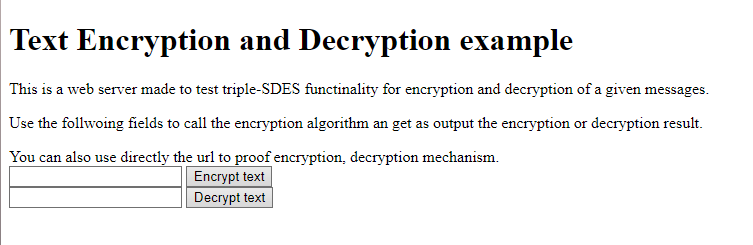
\includegraphics[width=0.8\textwidth]{assets/ServerIndex.png}
    \caption{A demo of the server created with the provided keys and mounted as a live tool to cipher and decipher text. }
    \label{fig:my_label}
\end{figure}

\begin{figure}
    \centering
    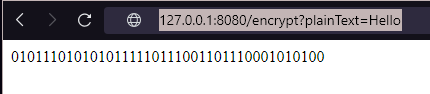
\includegraphics[width=0.8\textwidth]{assets/ServerCrypt.png}
    \caption{Server encryption example of the work 'Hello', obtaining the key '0101110101010111110111001101110001010100'. }
    \label{fig:my_label}
\end{figure}


\begin{figure}
    \centering
    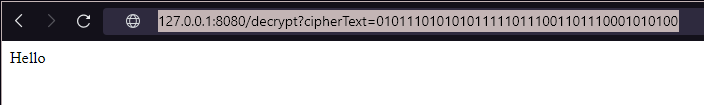
\includegraphics[width=0.8\textwidth]{assets/ServerDecrypt.png}
    \caption{Server decryption example of the bit-word '0101110101010111110111001101110001010100', obtaining the word 'Hello'. }
    \label{fig:my_label}
\end{figure}

\newpage

\section{Conclusion}
For this assignment different topics were analyzed and researched to produce insightful information and important understanding for the encryption algorithms for:
\begin{enumerate}
    \item \textbf{Polyalphabetic encryption algorithms}. It was possible to understand the way polyalphabetic ciphers work and the potential vulnerabilities for its simplicity by word substitution. It was demonstrated that even if the text is encoded in a different language, it would just be necessary to understand the word frequency distribution of such language to start with the brute-force attack.
    \item \textbf{SDES Algorithm}. Simple DES algorithm allowed a deep visualization, interpretation and understanding of encryption algorithms and schemes. Extremely important and useful being able to read and understand the technical SDES Sheet\cite{WS2017-SDES} and then translate it into code. Perform proper tests and finally give it a proper structure to make it part of a useful package. 
    \item \textbf{Triple DES Algorithm}. Very interesting to realize how by just repeating SDES algorithm and using different keys, the ciphering process can be strengthen 1000 times, making the deciphering mechanism even more complicated.
    \item \textbf{Server encryption and test}. After the implementation of a SDES algorithm it was possible to take it into a single module and use it to create a web server. Very interesting to realize that depending on the internet protocol (http or https), the submit mechanism (GET or POST) and the way the source code and keys are stored on the server side play an important role for secure systems. Being naive in its configuration, protection and proper storage might end up being very critical for any organization.
    \item \textbf{Statistical analysis, Cryptanalysis and brute-force algorithms}. Trying to find the different ways to analyze ciphered texts and perform statistical analysis involved very interesting approaches and knowledge acquired to create all the code and implementations to perform the cracking instructions and server mounting.
\end{enumerate}
All results have been packed and submitted into a repository where all the information and research can be found.

A very important lesson learned from this analysis is the realization that no system is 100\% secure, it is just matter of time and resources before one can access to relevant information, however, time and resources play a key role on it, so it is probable although unfeasible to break encryption algorithms.


\bibliographystyle{plainnat}
\bibliography{references}



\end{document}
